\documentclass[a4paper,11pt,twoside]{scrartcl}
\usepackage[T1]{fontenc}
\usepackage[utf8]{inputenc}
\usepackage{geometry}
\geometry{left=25mm, right=15mm, bottom=25mm}
\setlength{\parindent}{0em} 
\setlength{\headheight}{0em}
\usepackage{listings, textcomp}
\usepackage[usenames,dvipsnames,svgnames,table]{xcolor}


\definecolor{Code}{rgb}{0,0,0}
\definecolor{Keywords}{rgb}{0,0,255}
\definecolor{Strings}{rgb}{255,0,0}
\colorlet{Comments}{Green}
\colorlet{Numbers}{blue}

%%%%%%%%%%%
%Mache Integer farbig
%%%%%%%%%%%

\makeatletter

\newif\iffirstchar\firstchartrue
\newif\ifstartedbyadigit

\newcommand\processletter
{%
	\ifnum\lst@mode=\lst@Pmode%
	\iffirstchar%
	\global\startedbyadigitfalse%
	\fi
	\global\firstcharfalse%
	\fi
}

\newcommand\processdigit
{%
	\ifnum\lst@mode=\lst@Pmode%
	\iffirstchar%
	\global\startedbyadigittrue%
	\fi
	\global\firstcharfalse%
	\fi
}

\lst@AddToHook{Output}%
{%
	\ifstartedbyadigit%
	\def\lst@thestyle{\color{Numbers}}%
	\fi
	\global\firstchartrue%
	\global\startedbyadigitfalse%
}

\newtoks\jubo@toks
\jubo@toks={
	language=C,
	commentstyle=\color{Comments}\slshape,
	stringstyle=\color{Strings},
	keywordstyle={\color{Keywords}\bfseries},
	alsoletter=0123456789,
	SelectCharTable=%
}
\def\add@savedef#1#2{%
	\begingroup\lccode`?=#1\relax
	\lowercase{\endgroup
		\edef\@temp{%
			\noexpand\lst@DefSaveDef{\number#1}%
			\expandafter\noexpand\csname lsts@?\endcsname{%
				\expandafter\noexpand\csname lsts@?\endcsname\noexpand#2}%
		}}%
		\jubo@toks=\expandafter{\the\expandafter\jubo@toks\@temp}%
	}
	\count@=`0
	\loop
	\add@savedef\count@\processdigit
	\ifnum\count@<`9
	\advance\count@\@ne
	\repeat
	\count@=`A
	\loop
	\add@savedef\count@\processletter
	\ifnum\count@<`Z
	\advance\count@\@ne
	\repeat
	\count@=`a
	\loop
	\add@savedef\count@\processletter
	\ifnum\count@<`z
	\advance\count@\@ne
	\repeat
	%\showthe\jubo@toks % for debugging
	\begingroup\edef\x{\endgroup
		\noexpand\lstdefinestyle{pseudo}{\the\jubo@toks}
	}\x
	
	\makeatother
%%%%%%%%%%
%Ende
%%%%%%%%%%



\lstset{
	literate={ö}{{\"o}}1
	{ä}{{\"a}}1
	{ü}{{\"u}}1
	{ß}{{\ss}}1
	{/pi}{{$\Pi$}}1
	{/inf}{{$\infty$}}1
	{/eIn}{{$\in$}}1
	{/cup}{{$\cup$}}1
	{/leer}{{$\emptyset$}}1
	{<=}{{$\leq$}}1
	{>=}{{$\geq$}}1
	{→}{{$\rightarrow$}}1
	{⊈}{{$\not\subseteq$}}1
	{⊆}{{$\subseteq$}}1
	{∉}{{$\notin$}}1
	{∈}{{$\in$}}1
	{⇒}{{$\Rightarrow$}}1
	{∪}{{$\cup$}}1
	{α}{{$\alpha$}}1
	{∅}{{$\emptyset$}}1	
}


\lstset{
	numberstyle=\tiny,
	stepnumber=1,
	numbersep=10pt,
	xleftmargin=15pt,
	breaklines=true,
	numberblanklines=false,
	showstringspaces=false,
	flexiblecolumns=true,
	mathescape=true,
	tabsize=4,
	captionpos=b,
	numbers=left,
	commentstyle=\color{Green},
	numberstyle=\color{gray},
	keywordstyle=\color{blue} \textbf,%otherkeywords={xdata},
	keywords=[2]{xdata},
	keywordstyle=[2]\color{red}\textbf,
	identifierstyle=\color{black},
	stringstyle=\color{red}\ttfamily,
	basicstyle = \ttfamily \color{black} \footnotesize,
	inputencoding=utf8,
	emph=[1]%
	{%
		infinity,
	}, 
	emphstyle=[1]{\color{blue}},
	emph=[2]%
	{%
		forall,
		while,
		if,
		else,
		for,
		return,
		new,
		NULL,
		null,
		int, 
		double, 
		float,
		class,
		void,
		false, 
		true,
		FALSE,
		TRUE,
	}, 
	emphstyle=[2]{\color{Magenta}},
	emph=[3]{b0, b1, n0, n1},
	emphstyle=[3]{\color{black}}
}
\usepackage{float}
\usepackage[section]{placeins}
\usepackage{epstopdf}
\usepackage{wrapfig}
\usepackage{caption}
\usepackage{subcaption}
\usepackage{graphicx}
\usepackage{pgfplots}
\usetikzlibrary{plotmarks}
\usetikzlibrary{patterns}
\usetikzlibrary{decorations.pathmorphing}
\begin{document}
	\section{Aufgabe 1: Weighted-Circuit-Satisfiability(WCS) (5+5=10 Punkte)}
	\begin{figure}[H]
		\centering
		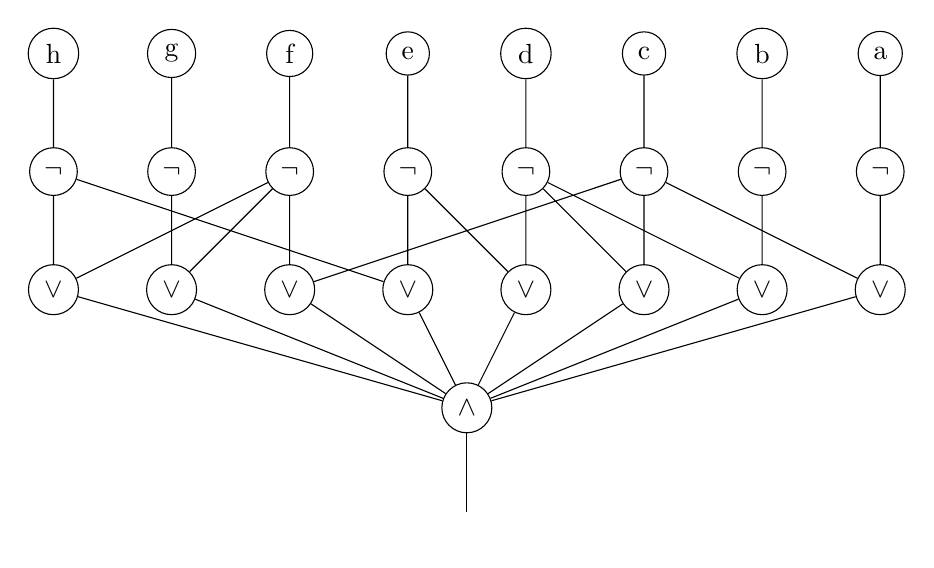
\begin{tikzpicture}[every node/.style = {draw, align=center, circle}, rotate = 180]
		\node[draw = white] {}
		child {
			node {$\land$}
			child {
				node (ac){$\lor$}
				child {
					node (a){$\neg$}
					child {node {a}}	
				}
			}
			child {
				node (bd){$\lor$}
				child {
					node (b){$\neg$}
					child{node {b}}	
				}
			}
			child {
				node (cd) {$\lor$}
				child {
					node (c) {$\neg$}
					child{node{c}}	
				}	
			}
			child {
				node (de) {$\lor$}
				child {
					node(d){$\neg$}
					child{node{d}}
				}	
			}
			child {
				node (eh) {$\lor$}
				child {
					node(e){$\neg$}
					child{node{e}}	
				}	
			}
			child{
				node (cf) {$\lor$}
				child {
					node (f) {$\neg$}
					child{node{f}}	
				}	
			}
			child {
				node (fg) {$\lor$}
				child {
					node(g) {$\neg$}
					child{node{g}}	
				}
			}
			child {
				node (fh) {$\lor$}
				child {
					node(h) {$\neg$}
					child{node{h}}
				}	
			}
		};
		\draw (c) -- (ac) (d)--(bd) (d) -- (cd) (e)--(de) (h)--(eh) (c)--(cf) (f)--(fg) (f)--(fh);
		\end{tikzpicture}
		\caption{a}
	\end{figure}
	\begin{figure}[H]
		\centering
		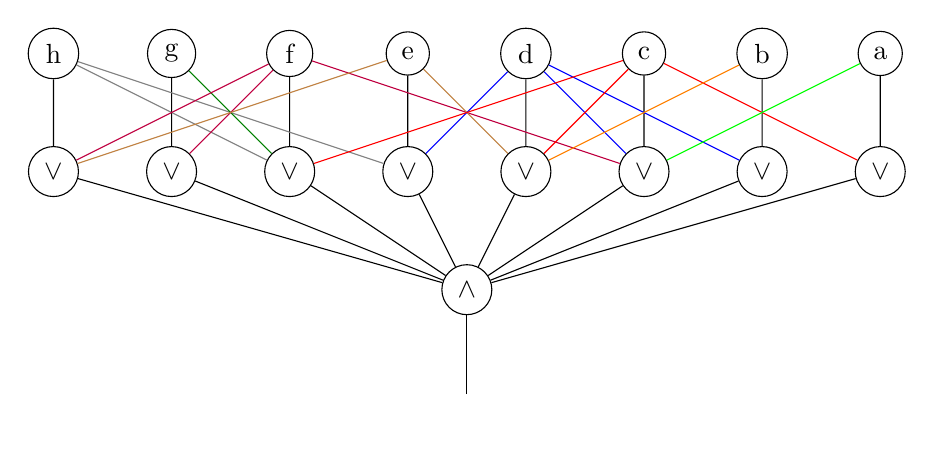
\begin{tikzpicture}[every node/.style = {draw, align=center, circle}, rotate = 180]
		\node[draw = white] {}
		child {
			node {$\land$}
			child {
				node (A) {$\lor$}
				child {
					node (a){a}	
				}
			}
			child {
				node (B){$\lor$}
				child {
					node (b) {b}	
				}
			}
			child {
				node (C){$\lor$}
				child {
					node (c){c}	
				}
			}
			child {
				node (D){$\lor$}
				child {
					node (d){d}	
				}
			}
			child {
				node (E){$\lor$}
				child {
					node (e){e}	
				}
			}
			child {
				node (F){$\lor$}
				child {
					node (f){f}	
				}
			}
			child {
				node (G){$\lor$}
				child {
					node (g){g}	
				}
			}
			child {
				node (H){$\lor$}
				child {
					node (h){h}	
				}
			}
		};
		\draw (c) edge[red] (A) (d) edge[blue] (B) (a) edge[green] (C) (f) edge[purple] (C) (d) edge[blue] (C) (c) edge[red] (D) (e) edge[brown] (D) (b) edge[orange] (D) (d) edge[blue] (E)	(h) edge[gray] (E) (c) edge[red] (F) (h)edge[gray](F) (g)edge[Green](F) (f)edge[purple](G) (f)edge[purple](H) (e)edge[brown](H);
		
		\end{tikzpicture}
		\caption{b}
	\end{figure}
\end{document}